\documentclass{paper}
\usepackage{graphicx}
\usepackage{url}
\usepackage[utf8]{inputenc}

\title{Research-Notes}
\author{Sameer Al Harbi}

\begin{document}
\part{deck.gl}
\today
\begin{quote}
\url{https://deck.gl/docs}
\end{quote}
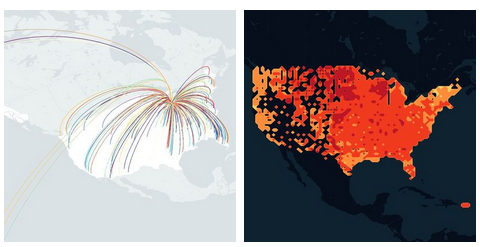
\includegraphics[width=180pt]{map2.PNG}
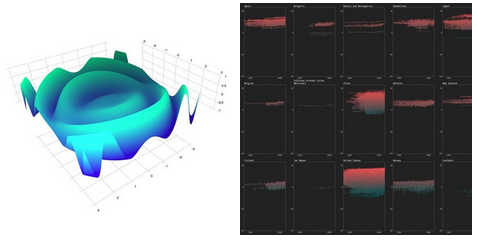
\includegraphics[width=180pt]{view.PNG}
\\
\\
deck.gl is a visualisation framework using WebGL for the analysis of large data sets. It mainly works by taking in JSON objects and building them into a stack of layers to create some impressive visual out of a very large number of data points. This is essentially an application that uses the GPU to visualize large number of data points in a accessible graphic. Layers allow usage of different visuals such as heat maps upon which you can add another layer like labels etc.. deck.gl seems to focus on geospatial data but is part of the vis.gl family of frameworks which all do roughly the same things but for different data

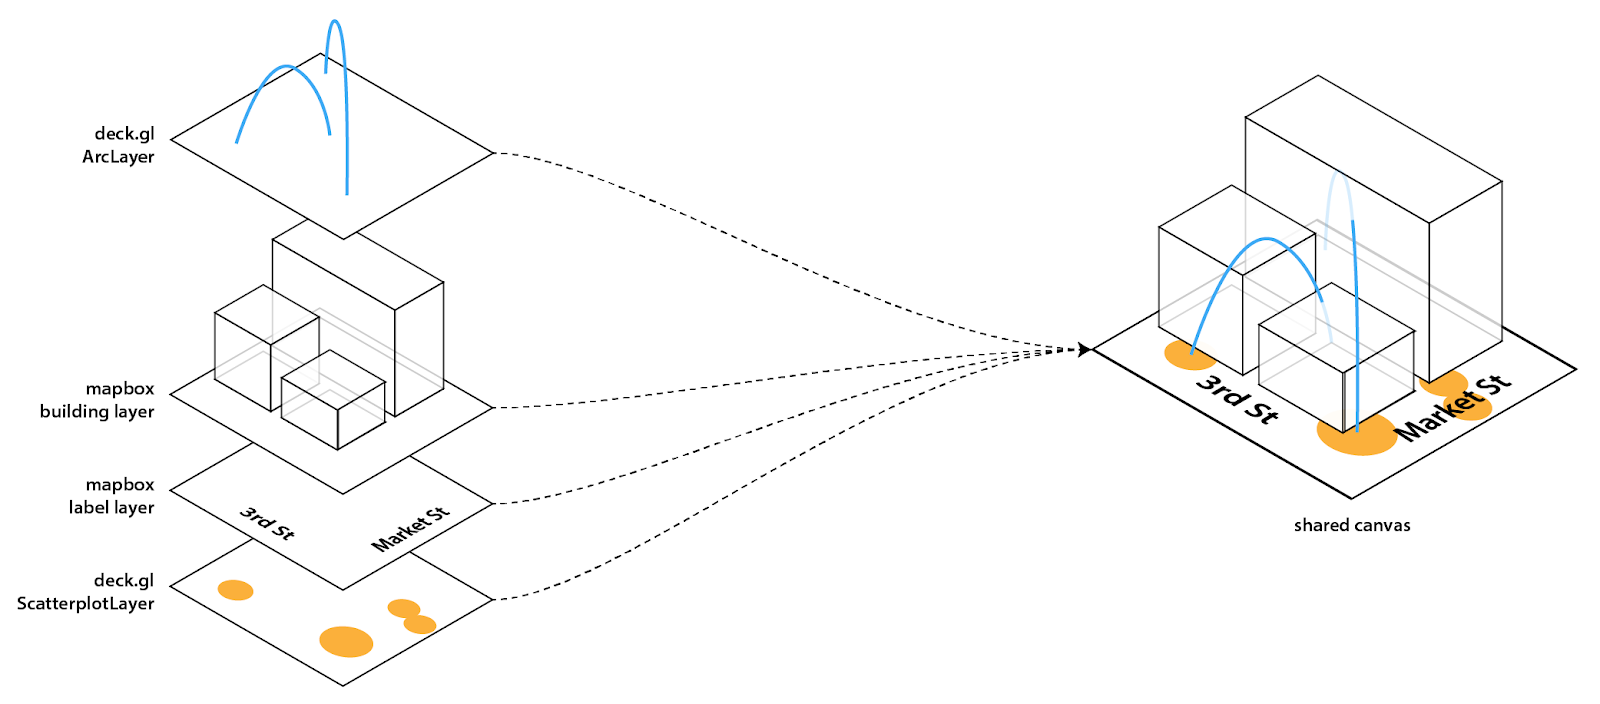
\includegraphics[width=220pt]{0 faYL1UbVD4af5qzy.png}
\\
\\
\textbf{Key Points to takeaway from this}
\begin{enumerate}
    \item Look Further into layers and see if something similar can be a useful pattern to adopt
    \item Consider the visualisation of the viewer, can different styles be used for different data? Maps? Cities? Maybe generators that based on data can create a visual. If city in data structure then generate map based on city points. Possibility for different camera views?
    \item Alternatively maybe premade views can be made, see the data on a globe or a map or on a classic 3D Graph
\end{enumerate}







\end{document}
